\documentclass[letterpaper, 10 pt, conference]{ieeeconf}  % Comment this line out
                                                          % if you need a4paper
%\documentclass[a4paper, 10pt, conference]{ieeeconf}      % Use this line for a4
                                                          % paper

\IEEEoverridecommandlockouts                              % This command is only
                                                          % needed if you want to
                                                          % use the \thanks command
\overrideIEEEmargins
% See the \addtolength command later in the file to balance the column lengths
% on the last page of the document



% The following packages can be found on http:\\www.ctan.org
\usepackage{graphicx} % for pdf, bitmapped graphics files
\graphicspath{{./images/}}
%\usepackage{epsfig} % for postscript graphics files
%\usepackage{mathptmx} % assumes new font selection scheme installed
%\usepackage{times} % assumes new font selection scheme installed
%\usepackage{amsmath} % assumes amsmath package installed
%\usepackage{amssymb}  % assumes amsmath package installed
\usepackage{listings}
\usepackage{url}

%%%%%%%%% JSON BEGIN %%%%%
\usepackage{xcolor}
\colorlet{punct}{red!60!black}
\definecolor{background}{HTML}{EEEEEE}
\definecolor{delim}{RGB}{20,105,176}
\colorlet{numb}{magenta!60!black}

\lstdefinelanguage{json}{
    basicstyle=\normalfont\ttfamily,
    numbers=left,
    numberstyle=\scriptsize,
    stepnumber=1,
    numbersep=8pt,
    showstringspaces=false,
    breaklines=true,
    frame=lines,
    backgroundcolor=\color{background},
    literate=
     *{0}{{{\color{numb}0}}}{1}
      {1}{{{\color{numb}1}}}{1}
      {2}{{{\color{numb}2}}}{1}
      {3}{{{\color{numb}3}}}{1}
      {4}{{{\color{numb}4}}}{1}
      {5}{{{\color{numb}5}}}{1}
      {6}{{{\color{numb}6}}}{1}
      {7}{{{\color{numb}7}}}{1}
      {8}{{{\color{numb}8}}}{1}
      {9}{{{\color{numb}9}}}{1}
      {:}{{{\color{punct}{:}}}}{1}
      {,}{{{\color{punct}{,}}}}{1}
      {\{}{{{\color{delim}{\{}}}}{1}
      {\}}{{{\color{delim}{\}}}}}{1}
      {[}{{{\color{delim}{[}}}}{1}
      {]}{{{\color{delim}{]}}}}{1},
}
%%%%%%%%%%%%%%%%%%%%JSON END %%%%

\title{\bf An Open Source Image Recognition Framework using Apache Tika and Tensorflow}

\author{Thamme Gowda$^{1,2,3}$ and Chris Mattmann$^{1,2,3}$% <-this % stops a space
\thanks{*This work was supported by DARPA MEMEX program}% <-this % stops a space
\thanks{$^{1}$University of Southern California, Los Angeles, CA }%
\thanks{$^{2}$NASA Jet Propulsion Laboratory, Pasadena, CA }%
\thanks{$^{3}$Apache Software Foundation, Non-Profit Organization}%
}
\begin{document}


\maketitle
\thispagestyle{empty}
\pagestyle{empty}


%%%%%%%%%%%%%%%%%%%%%%%%%%%%%%%%%%%%%%%%%%%%%%%%%%%%%%%%%%%%%%%%%%%%%%%%%%%%%%%%
\begin{abstract}
This paper describes uses of image recognition in content analysis, methods of integration and associated challenges and our final architecture of the system. //TODO: write this later as a summary of paper...
\end{abstract}


%%%%%%%%%%%%%%%%%%%%%%%%%%%%%%%%%%%%%%%%%%%%%%%%%%%%%%%%%%%%%%%%%%%%%%%%%%%%%%%%
\section{INTRODUCTION}
%% TODO: introduce Content Analysis and role in DARPA MEMEX
The objectives of Content Analysis are interpreting its meaning and establishing relationships \cite{}. Content analysis spreads across multimedia types like text in plain as well as rich formats, audio, image and video. //TODO: more here


Defense Advanced Research Projects Agency (DARPA) started a program called MEMEX\cite{} to help law keeping agencies to monitor and counteract the illegal activities on the web. The first challenge in such systems is to retrieve dark and deep content from the World Wide Web. Understanding the meaning and relationships are essential for performing various activities like filtering, classification, and ranking the severity etc. While humans can only efficiently and precisely analyze a small set of datasets, considering the scale of the dark and deep Web, automating the process is inherent requirement for its mission.

%% TODO: Introduce Tika and content analysis
Apache Tika\cite{mattmann2011tika} is a Free and Open Source (FOSS) content detection framework that can detect the patterns in raw content and determine its MIME and file type. It also has a rich pool of parsers, where its auto detection features can selectively apply sophisticated parsers based on the content type. However, reading or parsing content is a low level task compared to the high level task of interpreting the semantics of the content. In this paper we describe some useful enrichments to the framework that integrates recent innovations in the Artificial Intelligence (AI) domains to assist the automated content analysis. A vast majority of content on the web is in either plain or rich textual form \cite{}. Recently, Apache Tika added support for information extraction by the application of Natural Language Processing\cite{}. The newer version of Tika can be configured to recognize names in the content where it delegates the task to some of the popular Natural Language Processing toolkits. It supports various Named Entity Recognition(NER) techniques from toolkits like Stanford CoreNLP\cite{}, Apache OpenNLP\cite{}, MIT Lincoln Lab's MITIE \cite{}. Named Entity Recognition tasks from the text helps to briefly analyze the topics of the text. However, considering the fact that the image data on the web has the next biggest share, we historically lacked tools for automatically analyzing the graphical content without making much errors. 

%% TODO: Introduce the task of image/object recognition
Object recognition is a standard problem in computer vision which deals with the recognition of objects of interest in the graphical data. In the context of images it is often called as image recognition. Historically image recognition was a challenging task and its accuracy of the recognized objects were much lower than average Human performance. However, due to the recent advancements in deep neural networks and availability of larger datasets with faster computing resources, we now have systems which have nearer or better performance than average human beings.

%% TODO: introduce Image net

%% TODO: introduce Tensorflow

%% TODO: Describe the bigger challenge & Summarize how all these fit together
As of October 2016, the most popular deep learning frameworks are focused towards performance gain from native code and GPU optimization for fast matrix manipulations\cite{}. In our case, Tensorflow doesnot provide out of the box bindings to Java based frameworks. Apache Tika is primarily written in Java and thus integrating with Tensorflow is not straight forward like any other JVM compatible libraries. In this paper we explore various methods of integration and their pros and cons. 

%% brief overview of rest of the paper
The organization of the rest of this paper is as follows: Section \ref{sec:memex} provides an overview of the analysis task in which we describe data collection, analysis. Next, Section \ref{sec:obj-rec} describes the object recognition process and recent success with deep learning and the current state of the art model. Section \ref{sec:integration} covers various integration techniques we tried and the internal workings of it. Section \ref{sec:evaluation} provides pros and cons of each integration methods.

\section{CONTENT ANALYSIS IN MEMEX PROGRAM} \label{sec:memex}
This section discusses the background and motivations of DARPA Memex program and its datasets. The current commercial web search engines provides a generalized search interface to all users~\cite{}. However, in the context of cyber security, the commercial search engines miss resources from the deep and dark web which are essential for law keeping agencies. The goal of Memex program is to develop softwares that can quickly and thoroughly organize and search subsets of information relevant to the individual interests. The first two interests were in the domains of human trafficking and illegal weapon sale.
\subsection{Data Collection}
\label{sec:memex-datacollection}
Several web crawlers were used to discover and retrieve information from the websites. 
Along with the general purpose web crawlers, there were specialized crawler for the retrieval of dark data using TOR protocol \cite{} and also specialized in retrieval of dynamic AJAX content guarded by login forms. The fetched data were cached within the system for analysis due to the ephemeral nature of the content at the sources. 

\subsection{Memex Dataset} \label{sec:memex-dataset}
The dataset used in our experiment was a subset of memex dataset in public domain. It contained 7.2 million documents in the illegal weapon sales domain in which 1.4 documents were images. We had analyzed the textual documents and the named entities separately in a different experiment using named entity recognition models and extractors for people, location, organization, weapon-name and weapon-types. In this experiment we were interested in labeling images by classifying them into various classes. Usually web crawlers fetches all resources linked in the web pages and hences classification was an important pre-processing to remove noise for the later analysis.

\subsection{Visualization} \label{sec:memex-visualization}
A web interface was developed to browse the classified images in the index. //TODO: should we write about kyle's work here or not?

\section{OBJECT RECOGNITION} \label{sec:obj-rec}

\subsection{Deep Learning } \label{sec:deeplearning-imagenet}
\subsection{ImageNet} \label{sec:imagenet}

\subsection{Inception Network } \label{sec:inceptionnet}

\section{INTEGRATION} \label{sec:integration}
We defined an interface named \texttt{ObjectRecogniser} to facilitate multiple implementation of object recognizer. We developed the rest of the parsing framework against the \texttt{ObjectRecogniser} contract. The main part of this contract is a function that accepts image data and returns list of \texttt{RecognisedObject}s
%% TODO: Summarize the challenges
%% TODO: List the available methods
The following methods of integration were investigated in the order of listing:
\begin{itemize}
\item Command Line Invocation
\item Java Native Interface
\item gRPC Remote Procedure Calls
\item Representational State Transfer API 
\end{itemize}
%% TODO: Enumerate the methods, put figures, mention pros and cons
%% 1. CLI
\subsection{Command Line Invocation (CLI)} \label{sec:int-cli}
Command Line Invocation is the most simple way of integration. We created a python based CLI tool as an entry point to tensorflow's image recognition network. This tool inspected the environment for its requirements. When its requirements were not met it simply failed by reporting the failure. Some of its requirements were: 
\begin{enumerate}
\item NumPy
\item TensorFlow
\item Transitive dependencies of TensorFlow
\item Inception Net Model
\end{enumerate}
Apache Tika executed in the JVM process where as on every invocation of CLI tool, a new native process was created and destroyed.  Tika passed image path as commandline argument to the tool. The tool parsed the arguments, passed the content to tensorflow network and reported the results by printing it to standard output.  Tika parser then read the result from the output stream of this external process. The pros and cons are described in the Section \ref{sec:eval-cli}
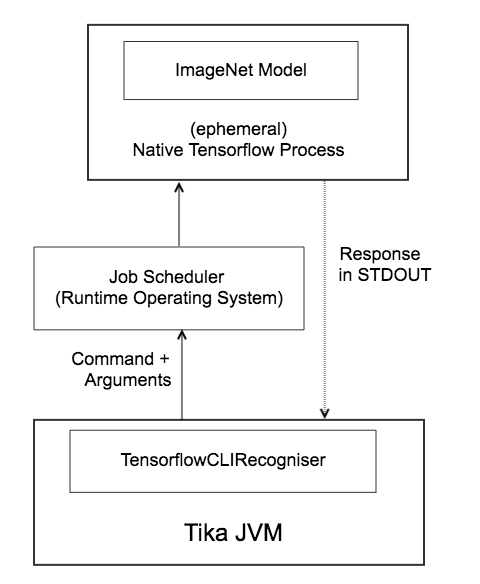
\includegraphics[scale=0.40]{tika-tflow-cli-design}

%% 2. JNI
\subsection{Java Native Interface (JNI)} \label{sec:int-jni}
The next approach we investigated was the Java Native Interface (JNI). JNI is the vendors' recommended way of integrating native code libraries to Java frameworks\cite{}. JNI acts as glue between bytecode instructions that runs within Java Virtual Machine (JVM) and the native  code instructions that runs directly on the CPU. Theoretically, this is the best way of merging JVM world with the native code\cite{}. At runtime, the bytecode of Tika (caller) and native code of tensorflow (callee) runs within the single process from the operating system's perspective. 

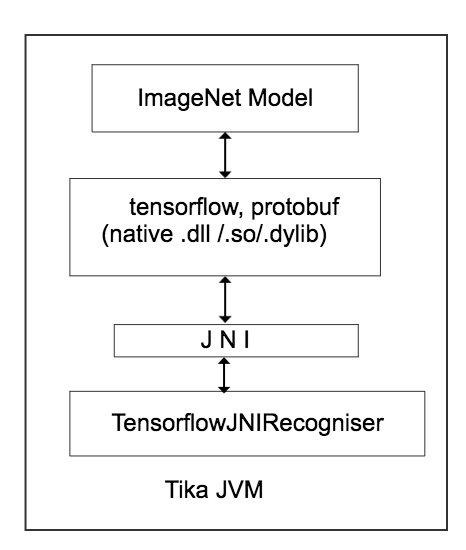
\includegraphics[scale=0.40]{tika-tflow-jni-design}

%% 3. RPC
\subsection{gRPC Remote Procedure Calls (gRPC)} \label{sec:int-rpc}
The original developers of Tensorflow framework recommended the use of gRPC based integration for the production systems\cite{}. gRPC is a client-server based architecture in which caller acts as a RPC client and callee serves as a server in a different address space. Unlike traditional RPC frameworks, gRPC is a high performance, CPU and bandwidth efficient transport on top of HTTP/2 that supports full duplex streaming\cite{}. In our case, we embedded gRPC client in Tika JVM and exported Tensorflow image recognition capabilities as remote procedures via gRPC service. We used Tensorflow Serving\cite{}, a gRPC\cite{} server implemented in C++, and also created a docker container to host it.

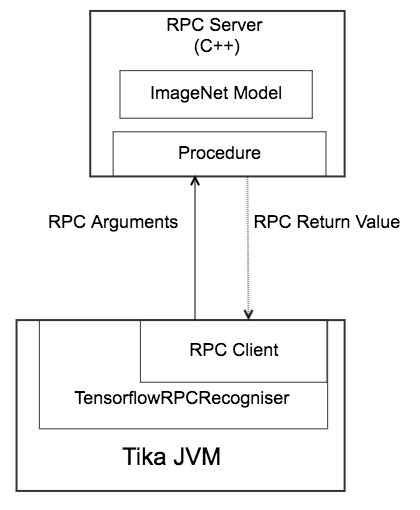
\includegraphics[scale=0.40]{tika-tflow-RPC-design}

%% 4. REST
\subsection{Representational State Transfer (REST) Application Programming Interface (API)} \label{sec:int-rest}
Representation State Transfer (REST) is a popular architecture paradigm for connecting heterogeneous system without the need of sessions\cite{}. The REST application programming interfaces (API) is powered by an HyperText Transfer Protocol (HTTP) which abstracts the complexities of Transmission Control Protocol.
We crated REST API for tensorflow image recognition using python Flask\cite{}. The Flask based HTTP service registered a TCP port from the operating system and offered HTTP API end points.
One of the end point was accepting a HTTP POST request with image data in the multipart form \cite{} body. This service loaded the InceptionNet \cite{} model during the initialization phase and kept the model in memory for reusing it during the future HTTP Requests. 

\begin{figure}[h]
    \centering
    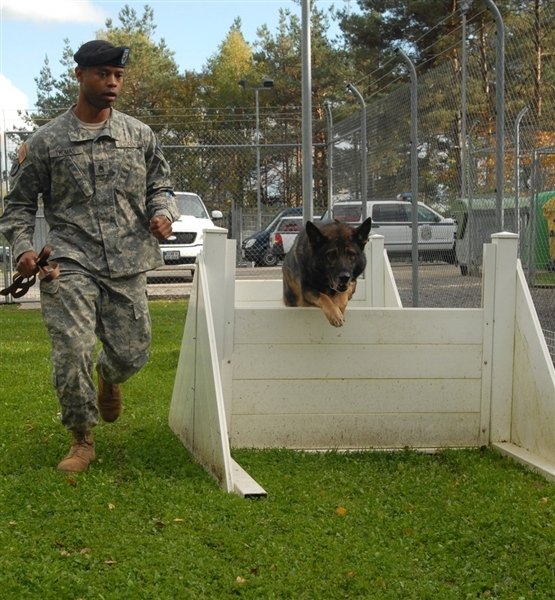
\includegraphics[scale=0.50]{military_dog}
    \caption{Military Person with a German Shepherd Dog \newline Courtesy: Wikimedia Commons}
    \label{fig:military-dog}
\end{figure}
The REST API, upon recognizing the objects in the image \ref{fig:military-dog}, returned the response in the JSON format with the following structure:

\begin{lstlisting}[language=json, label=code:json-output,
	frame=single, xleftmargin=5.0pt, xrightmargin=5.0pt,
    caption=JSON Response from REST API]
{
  "confidence": [
    0.3620266020298004,
    0.13061314821243286
  ],
  "classnames": [
    "German shepherd,
    German shepherd dog,
    German police dog, alsatian",
    "military uniform"
  ],
  "classids": [
    211,
    866
  ],
  "time": {
    "read": 1,
    "units": "ms",
    "classification": 257
  }
}
\end{lstlisting}

On the other side of the system, we implemented the class \texttt{TensorflowRESTRecogniser} which used HTTP Client to communicate with REST API. This implementation of \texttt{ObjectRecogniser} converted the image data to HTTP POST request with multipart form data and sent it to REST API. It parsed the JSON response to retrieve the object names, ids and confidence scores. We also created a docker specification for bootstrapping the tensorflow image recognition REST API for semi automated deployment of the system.

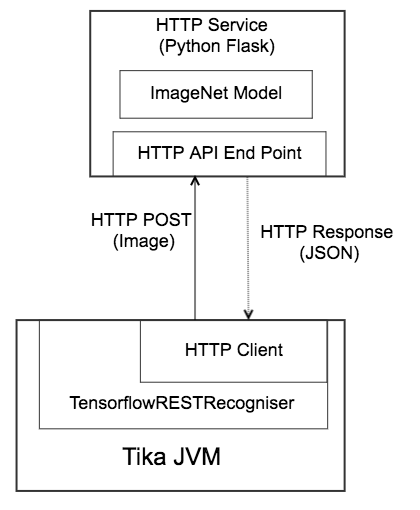
\includegraphics[scale=0.40]{tika-tflow-rest-design}


\section {EVALUATION} \label{sec:evaluation}
\subsection{Command Line Invocation (CLI)} \label{sec:eval-cli}
The average time taken to recognize image in this method was 6 seconds.

The pros of Command Line Interface:
\begin{itemize}
\item Easy to develop and test
\item Easy to install the requirements
\item Isolation of dependencies / concerns
\end{itemize}

The cons of this technique:
\begin{itemize}
\item The image data is shared via secondary storage which puts additional load on the  secondary storage.
\item An independent process is created and destroyed for every parse call.
\item The ImageNet model is loaded and unloaded for every parse call due to ephemeral nature of processes. The InceptionV3 model used in our experiments is approximately 200MB in size, thus 200MB of additional IO for each parse call.
\end{itemize}

%% 2. JNI
\subsection{Java Native Interface (JNI)} \label{sec:eval-jni}

The pros of this method are 
\begin{itemize}
\item The most efficient utilization of resources
\item No external input-output required as the entire task runs in a single process.
\end{itemize}

The cons of this method are:
\begin{itemize}
  \item The JNI glue code has to be compiled and packaged for all the platforms.
  \item Utilities like \texttt{protobuf} should also be glued with JNI, because they are required for deserializing models\cite{javacpp-240}. 
\end{itemize}

%% 3. RPC
\subsection{gRPC Remote procedure Call (gRPC)} \label{sec:eval-rpc}

The pros of this method are 
\begin{itemize}
\item An efficient way for integrating heterogeneous systems.
\item The client system is easily portable, server system can also be easily portable by making use of containerization or virtualization.
\end{itemize}

The cons of this method are:
\begin{itemize}
  \item The gRPC client may depend on specific versions of transitive dependencies such as HTTP Client which conflicts with existing functionality based on older HTTP Clients.
\end{itemize}

%% 4. REST
\subsection{Representational State Transfer (REST) Application Programming Interface (API)} \label{sec:eval-rest}

The average REST API call was 260 milliseconds when the client and server were in the same host (i.e., the connection via loopback interface).

The pros of this method are 
\begin{itemize}
\item An efficient and popular way for integrating heterogeneous systems.
\item The technology and practices are popular among developer community.
\item The underlying HTTP is stable and well documented.
\end{itemize}

The cons of this method are 
\begin{itemize}
\item The performance is slightly lower than gRPC.
\item Slightly higher bandwidth usage due to additional metadata introduced by HTTP to the packets.
\end{itemize}

\section{CONCLUSIONS}
%% TODO: link to Wiki page 

\section*{ACKNOWLEDGMENT}
This work was supported by the DARPA XDATA/Memex program. In addition, the NSF Polar Cyberinfrastructure award numbers PLR-1348450 and PLR-144562 funded a portion of the work. Effort supported in part by JPL, managed by the California Institute of Technology on behalf of NASA.

%%%%%%%%%%%%%%%%%%%%%%%%%%%%%%%%%%%%%%%%%%%%%%%%%%%%%%%%%%%%%%%%%%%%%%%%%%%%%%%%

\bibliographystyle{plain} % or try abbrvnat or unsrtnat
\bibliography{references} % refers to example.bib

\end{document}
